\documentclass[]{article}

\usepackage[utf8]{inputenc}
\usepackage[paperheight=0.9in,paperwidth=2.6in,margin=0in]{geometry}
\usepackage{tikz}
\usetikzlibrary{shapes,arrows,automata,calc}
\usepackage{color}

\usepackage{booktabs}  % nicer table borders 

\begin{document}

%\clearpage
%\thispagestyle{empty}

\tiny{
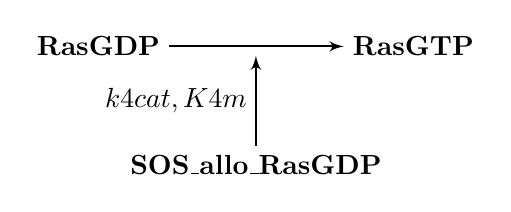
\begin{tikzpicture}[auto, outer sep=0pt, node distance=0cm,>=latex']

\node at (4, 0) (RAS_GTP) {$\bf RasGTP$};
\node at (0, 0) (RAS_GDP) {$\bf RasGDP$};
\node at (2, -1.5) (SOS_allo_RasGDP) {$\bf SOS\_allo\_RasGDP$};
\node at (2, 0) (MID) {};
    \draw [<-, thick] (RAS_GTP) to node {}
    (RAS_GDP);
    \draw [->, thick] (SOS_allo_RasGDP) to node {$k4cat, K4m$} (MID); 
\end{tikzpicture} 
}

\end{document}

